\documentclass[11pt,letterpaper]{article}

% Load some basic packages that are useful to have
% and that should be part of any LaTeX installation.
%
% be able to include figures
\usepackage{graphicx}
% get nice colors
\usepackage{xcolor}

% change default font to Palatino (looks nicer!)
\usepackage[latin1]{inputenc}
\usepackage{mathpazo}
\usepackage[T1]{fontenc}
% load some useful math symbols/fonts
\usepackage{latexsym,amsfonts,amsmath,amssymb}

% comfort package to easily set margins
\usepackage[top=1in, bottom=1in, left=1in, right=1in]{geometry}
\usepackage{hyperref}
\usepackage[all]{hypcap}
% control some spacings
%
% spacing after a paragraph\begin{figure}[bth]
\setlength{\parskip}{.15cm}
% indentation at the top of a new paragraph
\setlength{\parindent}{0.0cm}

\begin{document}

\begin{center}
\Large
Ay190 -- Worksheet 05\\
David Vartanyan\\
Date: \today
\end{center}

\section{Exercise 1}

\subsection{1a}
I used the data file emailed by Michael to plot Figure~\ref{fig:1}.

We will let x indicate log of stellar velocity dispersion $\sigma_*$ and y indicate log of black hole mass $M_{BH}$ in solar masses.


\subsection{1b}

See Figure~\ref{fig:2}.

Our best fit is

\begin{equation}
y=0.931069678177+ 1.27049767574\,x
\end{equation}

But wait! Green and Ho (2006) rescale x by $200 \,mathrm{km\, s}^{-1}$
After rescaling, my best fit is

\begin{equation}
y=7.66256957769+ 1.27049767574\, x
\end{equation} 

The intercept agrees fairly well with the data given in Green and Ho. The slope is small by a factor of 3.

\subsection{1c}

I used a left finite difference estimate for the derivative. In cases where we had multiple data points for a given value of x, I fixed the derivative at 0 so that it would remain finite. I also drop the last data point because we cannot extrapolate a left finite difference to these. Including errors roughly halves our intercept and slightly increases slope. See Figure~\ref{fig:3}.

Our best fit is 

\begin{equation}
y= 0.423118215597+ 1.38550311068\, x
\end{equation}

\begin{figure}[bth]
\centering
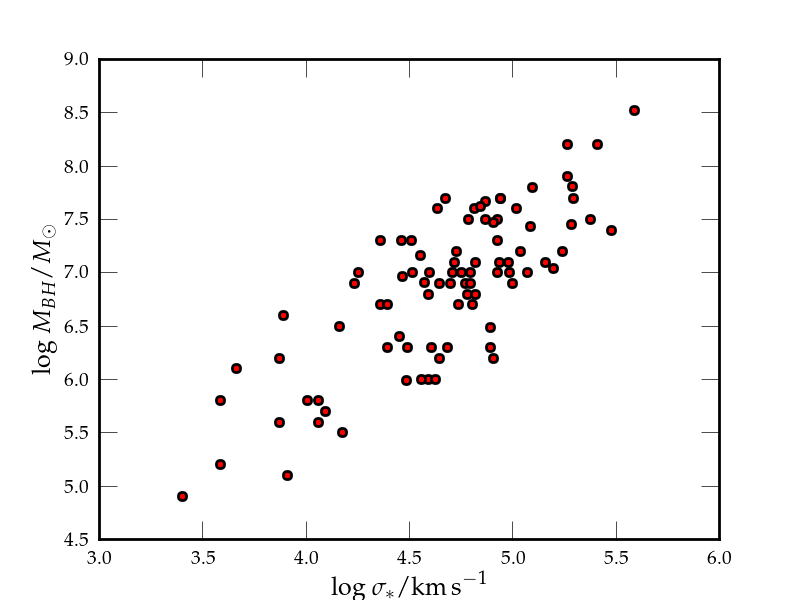
\includegraphics[width=0.7\textwidth]{ws5afig.png}
\caption{$M_{BH}\, \mathrm{vs}\, \sigma_*$ scatter.}
\label{fig:1}
\end{figure}

\begin{figure}[bth]
\centering
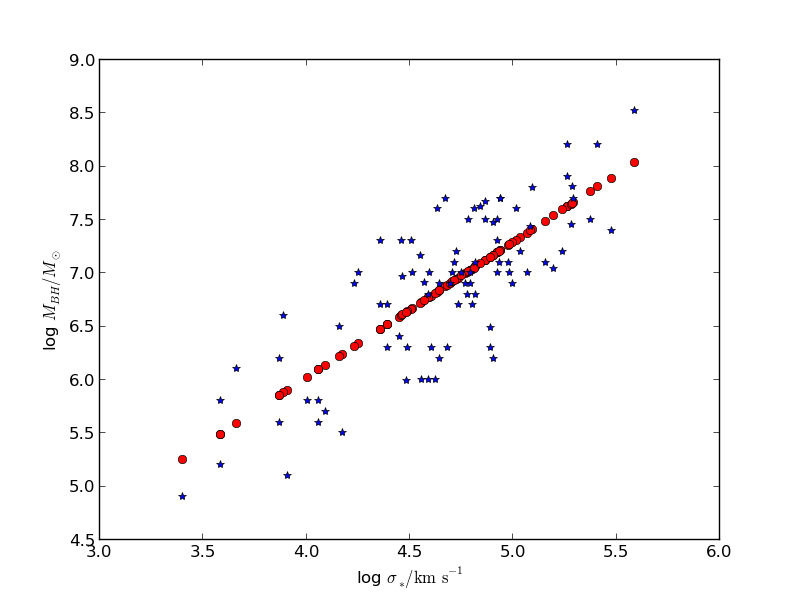
\includegraphics[width=0.7\textwidth]{ws5bfig.png}
\caption{Linear Fit, No Errors.}
\label{fig:2}
\end{figure}

\begin{figure}[bth]
\centering
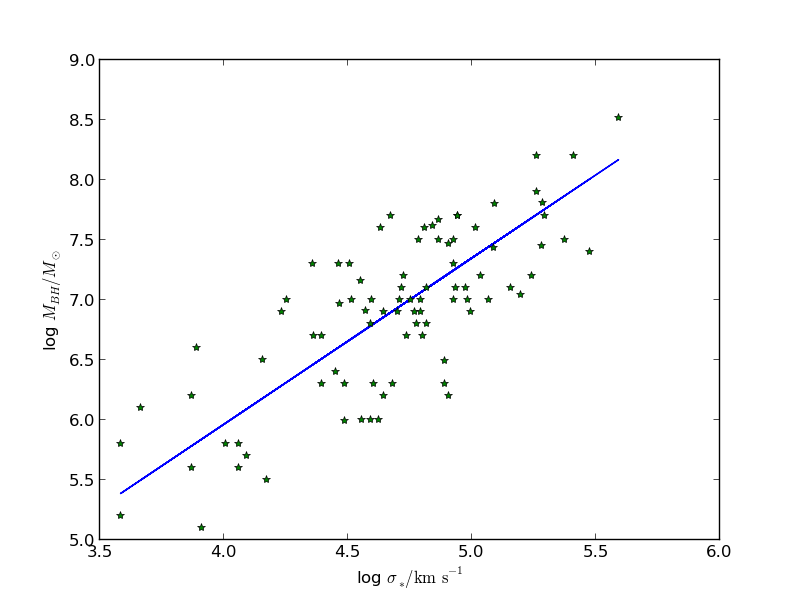
\includegraphics[width=0.7\textwidth]{ws5cfig.png}
\caption{Linear Fit Including Errors.}
\label{fig:3}
\end{figure}


\end{document}
